% === RDTs
\section{Resonance Driving Terms}

Decapoles, due to their order, contribute to many RDTs. Indeed, 50 of them can be theoretically 
observed in simulations and measurements. In practice, the contributions of individual RDTs
become indistinguishable as many resonances overlap, making it impossible to isolate certain terms.
Up to a fixed order, some resonances, described in~\cref{appendix:rdts}, are unique to
certain multipoles. Those resonances, provided that they are sufficiently strong and close to the
beam, can be measured via their RDTs.

Of interest to the LHC Operation, is the RDT $f_{1004}$, driving the resonance $1Q_x - 4Q_y$.
It can be seen in the horizontal frequency spectrum at $-4Q_y$ with an amplitude dependence on
$J_y^2$. 
Figure~\cref{fig:decapoles:rdts:tune_diagram} shows a frequency
map~\cite{yannis_papaphilippou_detecting_nodate} of a simulation including decapolar field errors,
where their impact on the beam is easily noticeable. The \todo{red} particles evolving close to the
resonance are affected by it and are subject to large tune shifts. Eventually, those particles are 
lost when their amplitude becomes too large.

\begin{figure}[H]
    \centering
    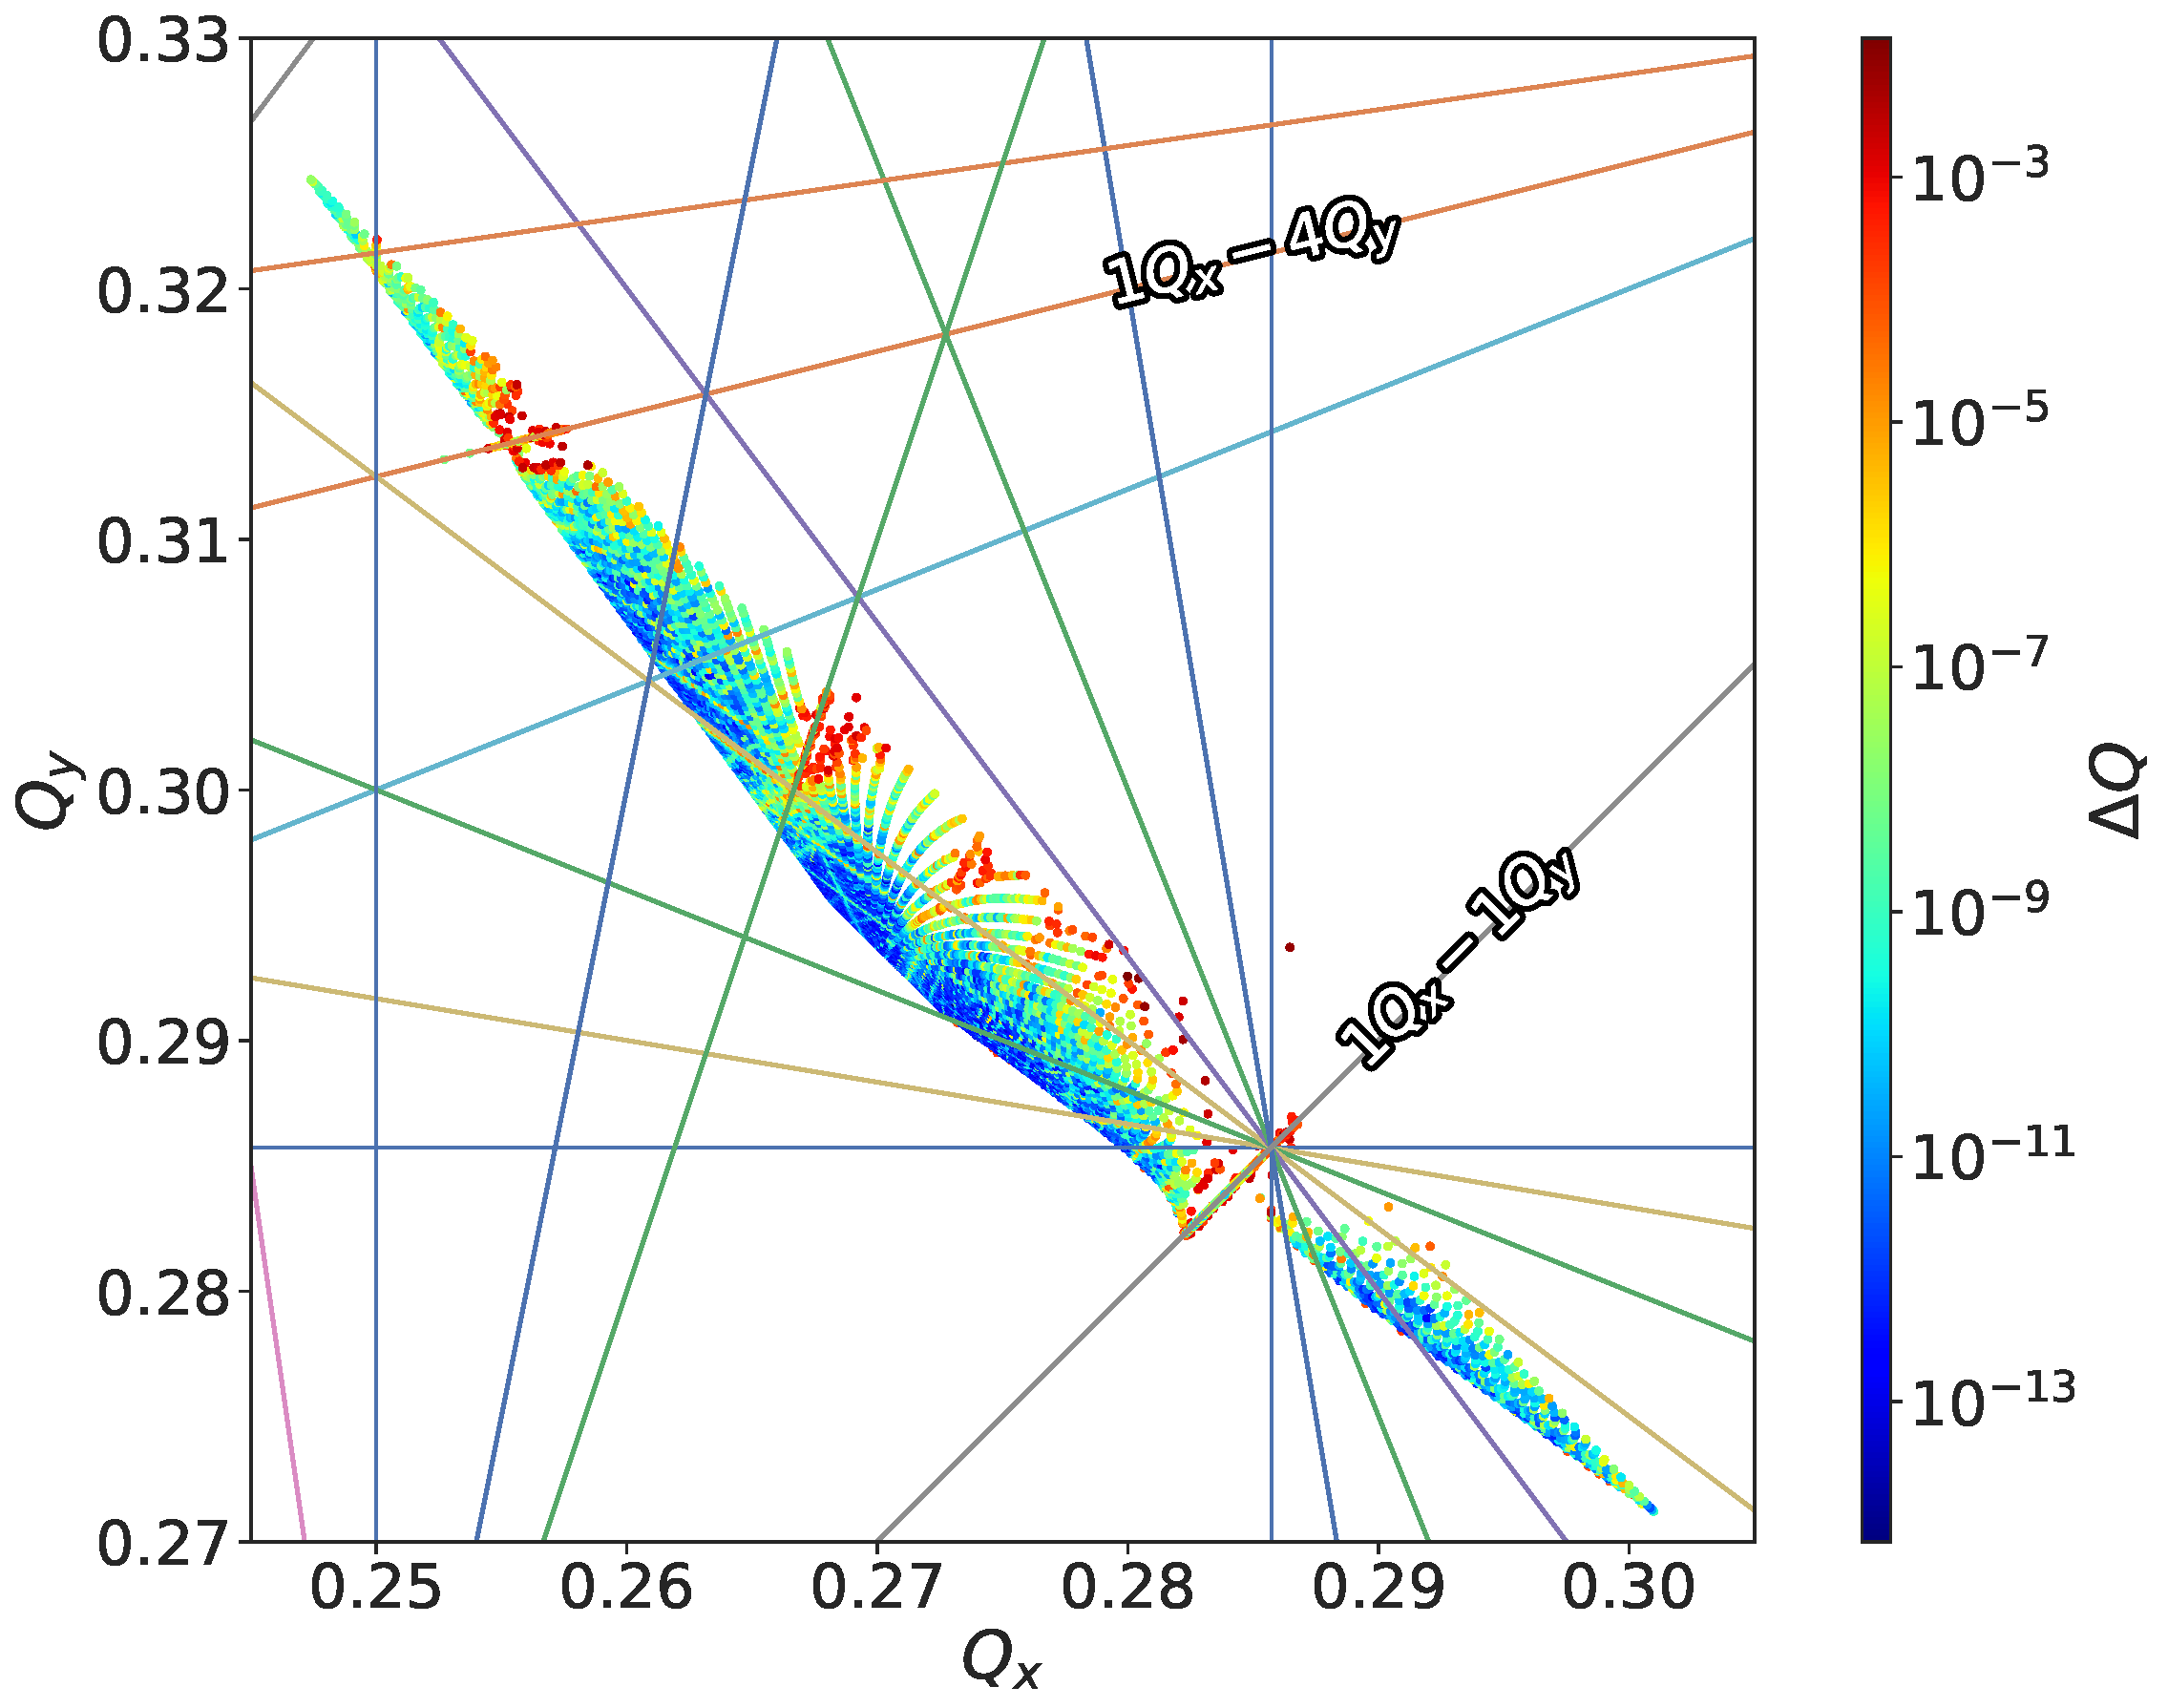
\includegraphics[width=1\textwidth]{./images/tune_diagram_f1004.pdf}
    \caption{Frequency map at injection energy, with decapolar field errors and nominal settings for
    landau octupoles. The highlighted resonance (1,-4), excited by decapoles, shows a degradation
    over 20,000 turns. The tune shift between the start and the end of the simulation is indicated
    in colour. \todo{change colormap}}
    \label{fig:decapoles:rdts:tune_diagram}
\end{figure}

Measuring turn-by-turn data without using any excitation is not a viable option as amplitudes are
not large enough. Spectral lines are indeed usually impossible to discern from the noise floor, 
making RDTs not measurable.
Measurements are hence taken with an AC-Dipole, introducing quadrupolar-like field errors in the 
linear regime~\cite{carlier_nonlinear_2020} and more complex effects in the non linear regime.
In practice, those effects are neglected. \textit{Forced} RDTs are measured with an
AC-Dipole and treated as \textit{free} as no compensation is applied.

Such forced measurements were taken for the first time in the LHC to observe the $f_{1004}$ RDT
at injection energy. The frequency line of the resonance $1Q_x - 4Q_y$ is seen at $4Q_y$ in the
horizontal spectrum, as shows \cref{fig:decapoles:rdts:spectrum_f1004}.

\begin{figure}[H]
    \centering
    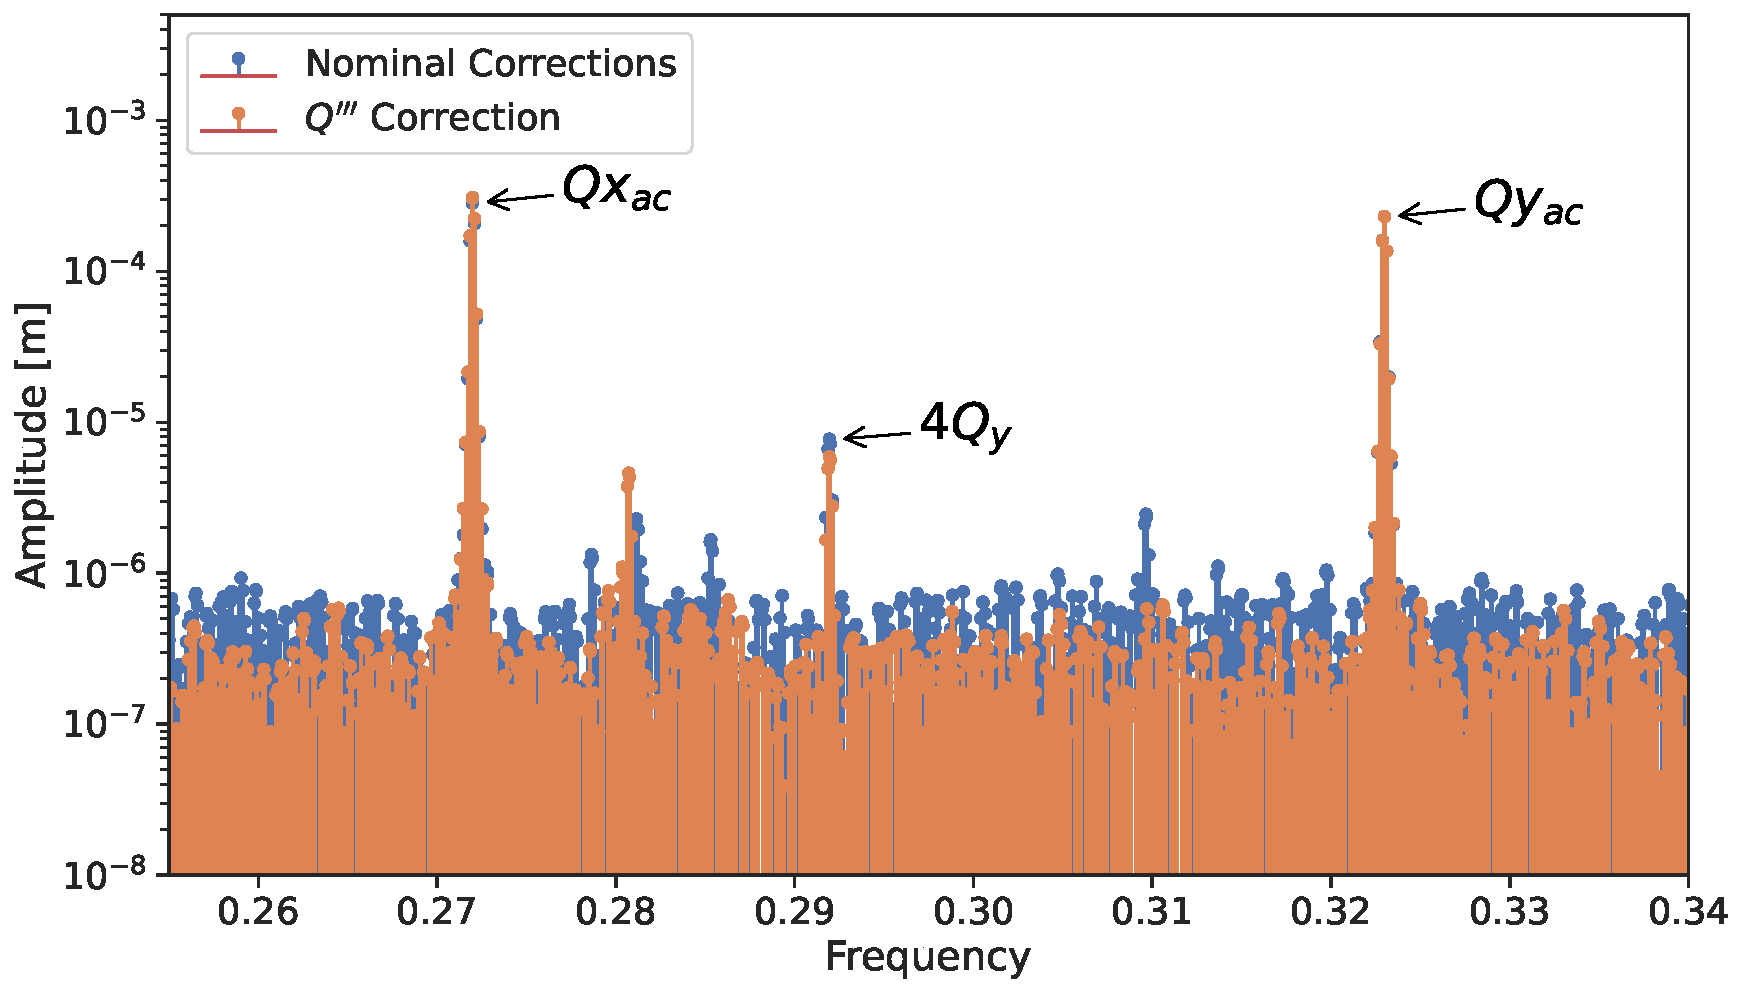
\includegraphics[width=0.9\textwidth]{./images/f1004x_spectrum.pdf}
    \caption{Horizontal frequency spectrum of turn-by-turn data, with nominal and beam-based
    corrections for the third order chromaticity $Q'''$. The $1Q_x - 4Q_y$ resonance can be seen
    at $-4Q_y$ with different amplitudes for each correction scheme.}
    \label{fig:decapoles:rdts:spectrum_f1004}
\end{figure}

Moreover, \cref{fig:decapoles:rdts:spectrum_f1004} shows that the amplitude of this resonance line
decreases upon application of beam-based corrections for $Q'''$. This translates to the amplitude
of the RDT $f_{1004}$, as seen in \cref{fig:decapoles:rdts:f1004_dq3}.

\begin{figure}[H]
    \centering
    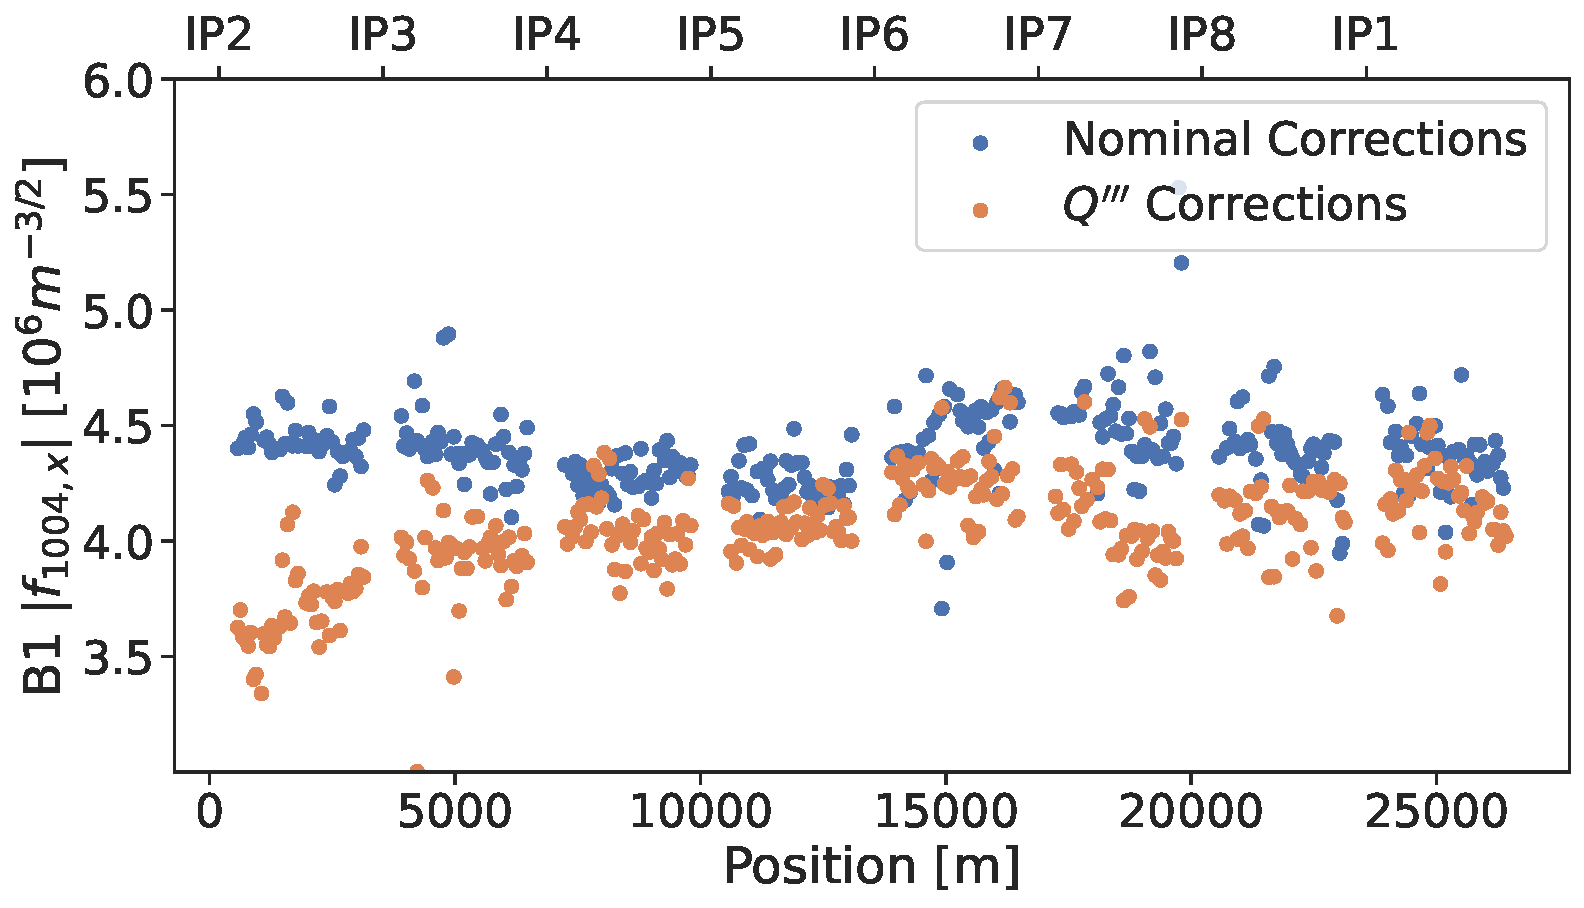
\includegraphics[width=0.9\textwidth]{./images/f1004_dq3.pdf}
    \caption{Amplitude of the RDT $f_{1004}$ generated by normal decapoles, measured before and
    after having applied beam-based corrections of the third order chromaticity $Q'''$.}
    \label{fig:decapoles:rdts:f1004_dq3}
\end{figure}


\todo{
    Measurements: \\
    \begin{itemize}
        \item 2022 Q'' and Q''' corrections 2022-04-24
        \item 2022-10-19 Virgin machine
        \item 2023-easter (FiDeL)
        \item 2023-06-14 MD9549 (FiDeL and Q'''/ RDT corr)
    \end{itemize}
    Effect of RCO correction on RDT f1004 \\
    Response
}

\subsection{Decapolar Contribution}

\subsection{Lower Order Contributions}